\documentclass[../../../../main.tex]{subfiles}

\begin{document}

\section*{東大理科 数学 1967 表紙・配点・概略}

\subsection*{難易度・分野一覧}
\begin{enumerate}
    \item 不等式 (難易度: A)
    \item 空間 (難易度: B)
    \item 多変数 (難易度: B)
    \item 関数 (難易度: B)
    \item 多変数 (難易度: A)
    \item 場合の数 (難易度: A)
\end{enumerate}

\newpage

\section*{第1問}

\noindent
[\textbf{解}] $x=0$ なら題意の成立は明白なので、以下 $x>0$ とする。$a>0$ とあわせて、AM-GM より、
\[
a x^{n+1} + \frac{1}{\sqrt[n]{a}} = a \cdot x^{n+1} + n \frac{1}{n \sqrt[n]{a}} \ge (n+1) \sqrt[n+1]{ a x^{n+1} \cdot \frac{1}{n^n a} }
\]
\[
= \frac{n+1}{n^{\frac{n}{n+1}}} x > x \quad \left( \because \frac{n+1}{n^{\frac{n}{n+1}}} > 1 \right) \quad \blacksquare
\]
となる。

\newpage

\section*{第2問}

\noindent
[\textbf{解}] 題意の“ある時刻”に自動車が原点にいるとし、自動車は $x$ 軸正方向へ動くものとする。また飛行機は平面 $z=k\ \text{[km]}\ (>0)$ 上をとるとする。
\[
\begin{cases}
A \cdots \text{“ある時刻”における飛行機の座標。} yz \text{平面上にとる。} \\
B \cdots 36 \text{秒後の} \qquad \qquad \text{〃} \\
C \cdots \qquad \quad \text{〃} \quad \text{自動車の座標}
\end{cases}
\]
とする。また点 $X$ に対し、$X$ の $xy$ 平面への正射影を $X'$ で表す。

\noindent
まず $\angle A O A' = 30^\circ$ から、$A(0, \sqrt{3}k, k)$ である。

\noindent
時速 $100\ \text{[km]} = \frac{10^5}{36}\ \text{[m/s]}$ ； $\sqrt{7} \times 100\ \text{[km/h]} = \frac{\sqrt{7} \cdot 10^5}{36}\ \text{[m/s]}$

\noindent
だから、$C(1, 0, 0)$ となる。題意から、
\[
B\left( 1 + \frac{3}{2}k, \frac{\sqrt{3}}{2}k, k \right)
\]
である。したがって、
\[
\vec{AB} = \begin{pmatrix} 1 + \frac{3}{2}k \\ -\frac{\sqrt{3}}{2}k \\ 0 \end{pmatrix}
\]
となる。$|\vec{AB}| = \sqrt{7}\ \text{[km]}$ だから、2乗して整理して、
\begin{align*}
7 &= \left(1 + \frac{3}{2}k\right)^2 + \left(\frac{\sqrt{3}}{2}k\right)^2 \\
  &= 3k^2 + 3k + 1
\end{align*}
\[
\therefore k = 1\ (>0)\ \text{[km]}
\]
したがって、求める高度は $k = 1000\ \text{[m]}$ である。

\begin{center}
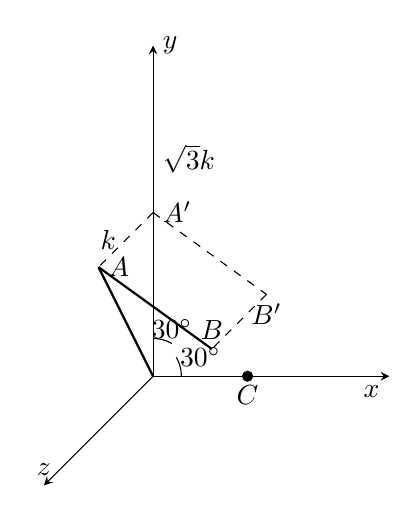
\begin{tikzpicture}[scale=1.2, >=stealth]
  % Axes
  \draw[->] (0,0,0) -- (2.5,0,0) node[below left] {$x$};
  \draw[->] (0,0,0) -- (0,3.5,0) node[right] {$y$};
  \draw[->] (0,0,0) -- (0,0,3) node[above] {$z$};

  % Points
  \coordinate (O) at (0,0,0);
  \coordinate (Ap) at (0, 1.732, 0);
  \coordinate (A) at (0, 1.732, 1.5);
  \coordinate (Bp) at (1.2, 0.866, 0);
  \coordinate (B) at (1.2, 0.866, 1.5);
  \coordinate (C) at (1.0, 0, 0);

  % Lines
  \draw[dashed] (O) -- (Ap);
  \draw[dashed] (Ap) -- (A);
  \draw[thick] (O) -- (A);
  \draw[dashed] (Bp) -- (B);
  \draw[thick] (A) -- (B);
  \draw[dashed] (Ap) -- (Bp);
  \draw[fill] (C) circle (1.5pt) node[below] {$C$};

  % Labels
  \node[right] at (A) {$A$};
  \node[right] at (Ap) {$A'$};
  \node[above] at (B) {$B$};
  \node[below] at (Bp) {$B'$};
  \node[left] at (0, 1.732, 0.75) {$k$};
  \node[right] at (0, 2.3, 0) {$\sqrt{3}k$};

  % Angle arcs
  \draw (0,0.4,0) arc (90:60:0.4);
  \node at (0.2,0.5,0) {$30^\circ$};

  \draw (0.3, 0, 0) arc (0:30:0.4);
  \node at (0.5, 0.2, 0) {$30^\circ$};
\end{tikzpicture}
\end{center}

\newpage

\section*{第3問}

\noindent
[\textbf{解}] $C = \cos\theta, S = \sin\theta$ とする。$A$ の周及び内部は、$A$ の中心 $(C,S)$ として、
\[
\begin{cases}
C-1 \le x \le C+1 \\
S-1 \le y \le S+1
\end{cases}
\quad \cdots \text{\raisebox{.5pt}{\textcircled{\raisebox{-.9pt}1}}}
\]
で表される。一方、$B$ の周及び内部は、
\[
\begin{cases}
0 \le x \le 2 \\
1 \le y \le 3
\end{cases}
\quad \cdots \text{\raisebox{.5pt}{\textcircled{\raisebox{-.9pt}2}}}
\]
で表される。これらが共通部分を持つ条件は $S \ge 0 \quad \cdots \text{\raisebox{.5pt}{\textcircled{\raisebox{-.9pt}3}}}$ で、この時、共通部分は
\[
\begin{cases}
0 \le x \le C+1 \\
1 \le y \le S+1
\end{cases}
\]
で表される。したがって、この面積 $T(\theta)$ として、
\[
T(\theta) = S(C+1)
\]
である。\raisebox{.5pt}{\textcircled{\raisebox{-.9pt}3}} 及び $C, S$ の周期性から、$0 \le \theta \le \pi$ で考えて良い。この時
\[
T'(\theta) = (2C-1)(C+1)
\]
から下表を得る。

\begin{center}
\begin{array}{c|c|c|c|c}
\theta & 0 & \frac{\pi}{3} & & \pi \\ \hline
T' & & + & 0 & - & 0 \\ \hline
T & & \nearrow & & \searrow &
\end{array}
\end{center}

\noindent
したがって、$\max T(\theta) = T\left(\frac{\pi}{3}\right) = \frac{3}{4}\sqrt{3}$ である。

\newpage

\section*{第4問}

\noindent
[\textbf{解}] $C : x^2 - xy + y^2 = 3$ とする。$C$ 上の点 $(x,y)$ を原点中心に $-\frac{\pi}{4}$ 回転した点 $(X,Y)$ とすると、
\begin{align*}
x + iy &= (X + iY) \left( \cos\left(-\frac{\pi}{4}\right) + i \sin\left(-\frac{\pi}{4}\right) \right) \\
       &= \frac{\sqrt{2}}{2} (1-i)(X + iY)
\end{align*}
\[
\therefore x = \frac{\sqrt{2}}{2}(X+Y), \quad y = \frac{\sqrt{2}}{2}(Y-X)
\]
だから、$C$ に代入して、
\[
\frac{1}{2}(X+Y)^2 + \frac{1}{2}(-X+Y)^2 - \frac{1}{2}(X+Y)(Y-X) = 3
\]
\[
\therefore \frac{X^2}{2} + \frac{Y^2}{6} = 1
\]
だから、$C$ は、楕円 $\frac{1}{2}x^2 + \frac{1}{6}y^2 = 1$ を原点中心に $-\frac{\pi}{4}$ 回転した図形で、右下図のようになる。

\noindent
ここで、右下図の斜線部の面積を求めれば良いので、この面積 $T$ として、$(X,Y) = \left( \frac{x}{\sqrt{6}}, \frac{y}{\sqrt{2}} \right)$ なる変換をすると、
\[
\frac{1}{\sqrt{6}}\frac{1}{\sqrt{2}} \cdot T = 2 \left[ \frac{1}{2} \cdot \frac{\pi}{3} \cdot 1^2 \right]
\]
\[
\therefore T = 2\sqrt{3} \frac{\pi}{3}
\]
が得られる。

\begin{center}
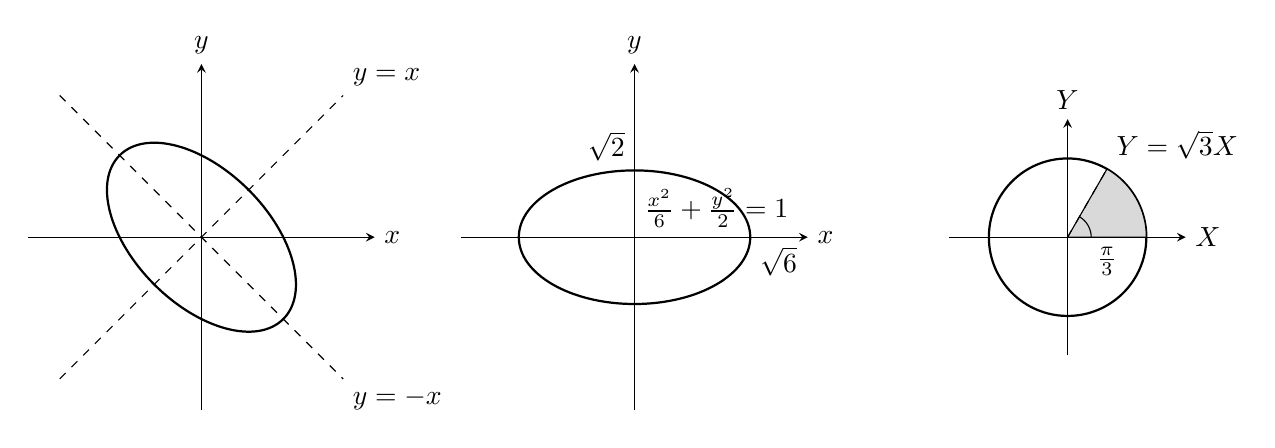
\begin{tikzpicture}[scale=1.0, >=stealth]
  % Rotated Ellipse figure
  \begin{scope}[shift={(0,0)}]
    \draw[->] (-2.2,0) -- (2.2,0) node[right] {$x$};
    \draw[->] (0,-2.2) -- (0,2.2) node[above] {$y$};
    \draw[rotate around={-45:(0,0)}, thick] (0,0) ellipse ({sqrt(6)*0.6} and {sqrt(2)*0.6});
    \draw[dashed] (-1.8,-1.8) -- (1.8,1.8) node[above right] {$y=x$};
    \draw[dashed] (-1.8,1.8) -- (1.8,-1.8) node[below right] {$y=-x$};
  \end{scope}

  % Aligned Ellipse figure
  \begin{scope}[shift={(5.5,0)}]
    \draw[->] (-2.2,0) -- (2.2,0) node[right] {$x$};
    \draw[->] (0,-2.2) -- (0,2.2) node[above] {$y$};
    \draw[thick] (0,0) ellipse ({sqrt(6)*0.6} and {sqrt(2)*0.6});
    \node[below right] at ({sqrt(6)*0.6},0) {$\sqrt{6}$};
    \node[above left] at (0,{sqrt(2)*0.6}) {$\sqrt{2}$};
    \node[above right] at (0,0) {$\frac{x^2}{6}+\frac{y^2}{2}=1$};
  \end{scope}

  % Transformed Circle figure
  \begin{scope}[shift={(11,0)}]
    \draw[->] (-1.5,0) -- (1.5,0) node[right] {$X$};
    \draw[->] (0,-1.5) -- (0,1.5) node[above] {$Y$};
    \draw[thick] (0,0) circle (1.0);
    \draw[fill=gray!30] (0,0) -- (1.0,0) arc (0:60:1.0) -- cycle;
    \node[below] at (0.5,0) {$\frac{\pi}{3}$};
    \draw (0.3,0) arc (0:60:0.3);
    \draw[dashed] (0,0) -- ({cos(60)},{sin(60)}) node[above right] {$Y=\sqrt{3}X$};
  \end{scope}
\end{tikzpicture}
\end{center}

\newpage

\section*{第5問}

\noindent
[\textbf{解}] $x=t\ (>0)$ で両者が接する時、$(\log x)' = \frac{1}{x}, \ (a x^2)' = 2ax$ より、
\[
\begin{cases}
a t^2 = \log t & \cdots \text{\raisebox{.5pt}{\textcircled{\raisebox{-.9pt}1}}} \\
2at = \frac{1}{t} & \cdots \text{\raisebox{.5pt}{\textcircled{\raisebox{-.9pt}2}}}
\end{cases}
\]
第2式より $at^2 = \frac{1}{2}$ だから、\raisebox{.5pt}{\textcircled{\raisebox{-.9pt}1}} に代入して
\[
\log t = \frac{1}{2} \quad \therefore t = e^{\frac{1}{2}} \quad \cdots \text{\raisebox{.5pt}{\textcircled{\raisebox{-.9pt}3}}}
\]
\raisebox{.5pt}{\textcircled{\raisebox{-.9pt}2}} に代入して
\[
a = \frac{1}{2t^2} = \frac{1}{2e} \quad \cdots \text{\raisebox{.5pt}{\textcircled{\raisebox{-.9pt}4}}}
\]
となる。このとき、求める面積 $S$ として
\begin{align*}
S &= \int_0^t a x^2 dx - \int_1^t \log x dx \\
  &= \frac{a}{3} t^3 - \Bigl[ x(\log x - 1) \Bigr]_1^t \\
  &= \frac{a}{3} t^3 - t(\log t - 1) + 1(-1) \\
  &= \frac{1}{6e} e \cdot e^{\frac{1}{2}} - e^{\frac{1}{2}} \left(-\frac{1}{2}\right) - 1 \quad (\because \text{\raisebox{.5pt}{\textcircled{\raisebox{-.9pt}3}}\text{\raisebox{.5pt}{\textcircled{\raisebox{-.9pt}4}}}) \\
  &= \frac{2}{3} e^{\frac{1}{2}} - 1
\end{align*}

\newpage

\section*{第6問}

\noindent
[\textbf{解}] 全てのとり出し方は ${}_9\mathrm{P}_9$ 通りで同様にたしからしい。

\noindent
一致する5枚のえらび方は ${}_9\mathrm{C}_5$ 通りで、たとえばこれが5〜9とすると、残りの4枚のならべ方は以下の通り (1または 左端が2の時。3,4の時も同じく3通りずつある)

\begin{center}
\begin{array}{c|c|c|c}
1 & 2 & 3 & 4 \\ \hline\hline
2 & 1 & 4 & 3 \\
2 & 3 & 4 & 1 \\
2 & 4 & 1 & 3
\end{array}
\end{center}

\noindent
したがって、このような並べ方は
\[
{}_9\mathrm{C}_5 \cdot 3 \times 3 = 9 \cdot {}_9\mathrm{C}_4 \text{ 通り}
\]
である。したがって、求める確率は
\[
\frac{9 \cdot {}_9\mathrm{C}_4}{{}_9\mathrm{P}_9} = \frac{\frac{9 \cdot 8 \cdot 7 \cdot 6}{4 \cdot 3 \cdot 2 \cdot 1}}{8 \cdot 7 \cdot 6 \cdot 5 \cdot 4 \cdot 3 \cdot 2} = \frac{1}{320}
\]

\end{document}
